\documentclass[a4paper,11pt]{article}

\usepackage[utf8]{inputenc}
\usepackage[a4paper, left=3cm, right=3cm, top=3cm, bottom=3cm]{geometry}
\usepackage[frenchb]{babel}
\usepackage{default}
\usepackage{pslatex}
\usepackage{graphicx}
\usepackage{algorithmic}
\usepackage{multicol}
\usepackage{amsmath}
\usepackage{amssymb}
\usepackage{textcomp}
\usepackage{pgf}
\usepackage{tikz}
\usepackage{pgfplots}
\usepackage{capt-of}
\usepackage{esvect}
\usepackage[T1]{fontenc}
\usepackage[babel=true]{csquotes}
\usepackage{gensymb}

% \setcounter{tocdepth}{4}

%opening
\title{Tropodrone}
\author{Thibaut Manceau, Alexis Gros, Noé Gueydan, Tristan Porteries}

\begin{document}

\begin{Huge}
\maketitle
\end{Huge}

\clearpage

\tableofcontents

\clearpage

\section{Introduction}

\subsection{Besoins}

\subsection{Applications}

\subsection{Contraintes}

\subsubsection{Légalité}

\subsubsection{Drone}


\section{Étude de conception}

\subsection{Ballon}

\subsubsection{Élévation}

Le tropodrone doit utiliser un moyen de supporter une partie du poids du drone sans dépenser d'énérgie dans le but d'augmenter l'autonomie, pour ce faire nous utilisons la poussée d'Archimède d'un gaz plus léger que l'air. Comme ce gaz est plus léger que l'air la somme de son poids et de sa poussée d'Archimède forment une force verticale orienté vers le haut.

\paragraph{Archimède}

La poussée d'archimède est définie par~:

\enquote{Tout corps plongé dans un fluide au repos, entièrement mouillé par celui-ci ou traversant sa surface libre, subit une force verticale, dirigée de bas en haut et opposée au poids du volume de fluide déplacé ; cette force est appelée poussée d'Archimède.}

\begin{center}
	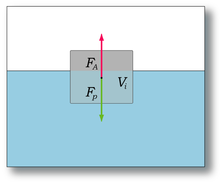
\includegraphics[width=5cm]{../Images/pousse_archimede.png}
\end{center}

Cette force se calcule avec la formule~:

\begin{center}
  \boxed{\vv{Fa} = -M_F \times \vv{g}}
\end{center}

Où $\vv{Fa}$ est la poussée d'archimède en $N$, $M_F$ la masse du fluide contenue dans le volume déplacé en $kg$, $\vv{g}$ la valeur du champ de pesanteur en $N.kg^{-1}$. \\

Un ballon de gaz est donc soumis à deux forces~: son poids et sa poussée d'Archimède~:

\begin{center}
  \boxed{\vv{F_{ballon}} = \vv{P_{ballon}} + \vv{Fa_{ballon}}}
\end{center}

Où $\vv{F_{ballon}}$ est la force d'élévation du ballon en $N$, $\vv{P_{ballon}}$ le poids du ballon en $N$, $\vv{Fa_{ballon}}$ la poussée d'Archimède éxercée sur le ballon en $N$. \\

Nous pouvons remarquer que si $P_{ballon} < Fa_{ballon}$ alors il existe une force d'élévation orienté vers le haut. De même cette force sera toujours  plus petite que la poussée d'Archimède éxercée sur le ballon, comme le ballon et le gaz possède toujours une masse~: $F_{ballon} < Fa_{ballon}$.
Par la suite on appellera capacité d'élevation la masse que peut supporter la force d'élévation d'un ballon~:
\begin{center}
	\boxed{Ca_{ballon} = \frac{F_{ballon}}{g}}
\end{center}

Où $Ca_{ballon}$ est la capacité d'élévation en $kg$, $F_{ballon}$ la force d'élévation en $N$ et $g$ la valeur du champ de pesanteur en $N.kg^{-1}$.

\paragraph{Gaz}

Pour avoir un gaz plus léger que l'air il faut qu'il est une masse volumique inférieur à celle de l'air~: $1.29kg.m^3$. Plusieurs gazs remplissent cette condition, les plus courants sont l'hélium est l'hydrogène dont les masse volumique et les capacités d'élévation calculées sont~:

\begin{center}
	\begin{tabular}{|l|c|c|c|}
		\hline
		Gaz & Air & Hydrogène & Hélium \\
		\hline
		Masse Volumique $(kg.m^3)$ & 1.29 & 0.08988 & 0.1785 \\
		\hline
		Force d'élévation $(N.m^3)$ & 0 & 11.77 & 10.90 \\
		\hline
	\end{tabular}
\end{center}

Le gaz retenu et l'hélium car il ne présente pas de rique de combustion contrairement à l'hydrogène, même si sa masse volumique est plus importante et que sa procuration est plus compliquée.

\paragraph{Dilatation}

En prenant exemple sur les montgolfières nous avons cherché à connaitre le gain de volume que pourrait avoir l'hélium à une température élevée. Ce gain de volume apporte directement une reduction de la masse volumique et donc l'augmentation de la force d'élévation.

La loi de Charles permet de calculer la dilatation d'un gaz. D'après Charles il existe un rapport volume température constant dépendent seulement de la pression du gaz et de la quantité de matière du gaz étudié.

\begin{center}
 \boxed{\displaystyle{\frac{V_1}{T_1} = \frac{V_2}{T_2} = f(P, n)}} \\
 $\displaystyle{V_3 = f(P, n) \times T_3}$
\end{center}

Où $V_n$ est le volume du gaz en $m^3$ à la température $T_n$ en $K$, $P$ la pression du gaz en $Pa$, $n$ la quantité de matière en $mol$ et $f(P, n)$ le rapport constant entre volume et temperature en $m^3.K^{-1}$.

L'application de cette loi à l'hélium à une température de $200 \degree C $ donne les résultats suivants~: \\

Le volume molaire de l'hélium est~: $22.414\times 10^{-3} m^3.mol^{-1}$ à $273.25K$. \\

\begin{center}
	$\displaystyle{f(P, n) = \frac{22.414\times 10^{-3}}{273.25} = 8.2\times 10^{-5} m^3.mol^{-1}.K^{-1}}$
	\bigbreak
	$T_{200} = 200 \degree C = 473.25K$
	\medbreak
	$\displaystyle{V_{T_{200}} = 8.2\times 10^{-5} \times 473.25 = 38.811 \times 10^{-3}} m^3.mol^{-1}$
\end{center}

Donc à $200 \degree C$ l'hélium a un volume molaire de $38.811 \times 10^{-3} m^3.mol^{-1}$ équivalent à 1.59 fois son volume molaire d'origine. Malgrés cette augmentation de volume, la force d'élévation varie peu car la poids de l'hélium est très faible et que la reduction de celui ci ne fera que ce rapprocher de la poussée d'Archimède~: \\

\begin{center}
  $\displaystyle{F_{T_0} = Fa_{air} - P_{helium} = 10.90 N}$
  \bigbreak
  $\displaystyle{F_{T_{200}} = Fa_{air} - \frac{P_{helium}}{1.59} = 11.57 N}$ \\
\end{center}

$F_{T_{200}} = 1.06 \times F_{T_0}$

À cause des faibles résultats obtenus et des problèmes introduits par la mise en oeuvre du chauffage d'un gaz~: résistance de l'enveloppe du ballon~; résistance de chauffage~; alimentation de la résistance. Cette idée est donc abandonnée.

\subsubsection{Enveloppe}

\paragraph{Materiaux}

\paragraph{Étanchéité}

\subsubsection{Collage}

\paragraph{Résistance}

\subsection{Structure}

\subsubsection{Étude des mouvements}

\subsubsection{Support ballon}

\subsection{Support drone}

\paragraph{1er modèle}

\paragraph{2ème modèle}


\section{Aérodynamisme}

\subsection{Influence sur la structure}

\subsubsection{Optimisation avec la forme en triangle}

\subsubsection{Gouvernail}

\subsection{Équation de trainée}

\subsubsection{Calcul du Cx}

\paragraph{Simulation SW}
!= conformations

\subsection{Simulation Python}


\section{Réalisation}

\end{document}
